\documentclass[UTF8]{ctexart}
\usepackage{amsmath}
\usepackage{graphicx}
\usepackage{minted}

\graphicspath{ {images/} }

\title{数据结构第一次作业}
\date{2016-9-30}
\author{软件51 沈俞霖 2151601013}

\begin{document}
  \maketitle
  \newpage

  \section{复杂度与时间估计}
    \subsection{作业题目}
      程序A和程序B经过分析发现其最坏情形运行时间分别不大于 $150N\log N$ 和 $N^2$ 。如果可能,请回答下列问题:
      \paragraph{A}
      对于 $N$ 的大值( $N>10000$ ),哪一个程序的运行时间有更好的保障?
      \paragraph{B}
      对于 $N$ 的小值( $N<100$ ),哪一个程序的运行时间有更好的保障?
      \paragraph{C}
      对于 $N=1000$ ,哪一个程序平均运行得更快?
      \paragraph{D}
      对于所有可能的输入,程序B是否总比程序A运行得快?
    \subsection{问题分析}
      \paragraph{A}
      A程序运行时间有更好的保障。当 $N=10000$ 时,在最坏情况下, $ 150 N \log N \approx 2 \times 10 ^ 7 $ , 而 $ N^2 = 10 ^ 8 $, 故A程序运行时间有更好的保障。
      \paragraph{B}
      B程序运行时间有更好的保障。当 $N=100$ 时,在最坏情况下, $ 150 N \log N \approx 10 ^ 5 $ , 而 $ N^2 = 10 ^ 4 $, 故B程序运行时间有更好的保障。
      \paragraph{C}
      不能判断,因为题目只给出了最坏情况运行时间,没有给出平均情况运行时间。
      \paragraph{D}
      不能判断,因为题目只给出了最坏情况运行时间,不能以此来判断所有的输入。
  \section{递归方程求复杂度}
    \subsection{作业题目}
      考虑以下递归方程,定义函数 $T(n)$ :
      \paragraph{A}
      \begin{equation}
        T(n) =
        \begin{cases}
          1, & \text{如果$n=1$} \\
          T(n - 1) + n, & \text{其他情况}
        \end{cases}
      \end{equation}
      \paragraph{B}
      \begin{equation}
        T(n) =
        \begin{cases}
          1, & \text{如果$n=0$} \\
          2T(n - 1), & \text{其他情况}
        \end{cases}
      \end{equation}

      请给出A和B两种递归式的大O表示,并证明。
    \subsection{问题分析}
      \paragraph{A}
        $T(n) = O(n^2)$

        \subparagraph{证明}

        (1) 令 $n = 1$,
        $$T(n) = 1 = \frac {n^2 + n}{2}$$

        (2) 若
        $$T(k) = \frac {k^2 + k}{2}$$
        则 $T(k + 1) = T(k) + k + 1$, 即
        $$T(k + 1) = \frac {(k + 1)^2 + (k + 1)}{2}$$

        由(1)(2)可知,
        $$T(n) = \frac {n^2 + n}{2}$$
        故 $T(n) = O(n^2)$,证毕。

      \paragraph{B}
        $T(n) = O(2^n)$

        \subparagraph{证明}

        (1) 令 $n = 0$,
        $$T(n) = 1 = 2 ^ n$$

        (2) 若
        $$T(k) = 2 ^ k$$
        则 $T(k + 1) = 2T(k)$, 即
        $$T(k + 1) = 2 ^ {k + 1}$$

        由(1)(2)可知,
        $$T(n) = 2 ^ n$$
        故 $T(n) = O(2 ^ n)$,证毕。
  \section{测试排序算法}
    \subsection{作业题目}

    实现直接插入排序、简单选择排序、希尔排序、快速排序和归并排序,以能够对给定数组的正序排序,并按照满足下列情形进行测试:

      \paragraph{A} 测试数组的大小为[100,200,300,…,10000] 100 种大小

      \paragraph{B} 测试数组中的元素分别为正序、逆序和随机序列

      \paragraph{} 对测试的结果需要用图形的方式进行展示:

        \subparagraph{a} 展示每个排序算法在满足条件 A 和条件 B 情形下的运行时间趋势变化图,如图 1 所示

        \begin{figure}[H]
          \caption{对选择排序的分析}
          \centering
          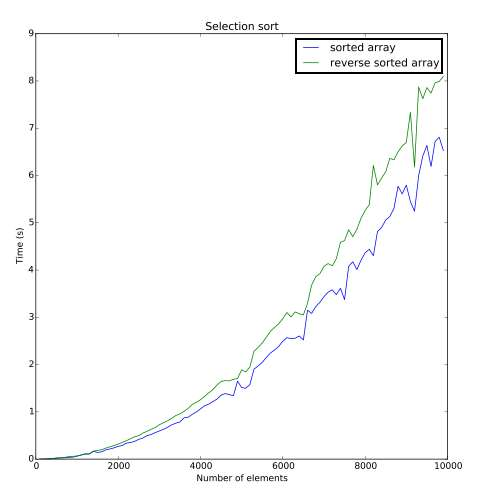
\includegraphics[width=0.5\textwidth]{example1}
        \end{figure}

        \subparagraph{b} 将所有排序算法在正序下、逆序下和随机序列下的运行时间的对比图,如图 2 所示

        \begin{figure}[H]
          \caption{对逆序排序的分析}
          \centering
          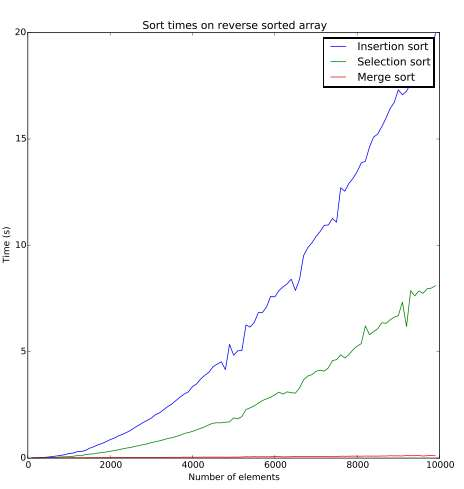
\includegraphics[width=0.5\textwidth]{example2}
        \end{figure}

    \subsection{程序实现}
      \paragraph{插入排序}
      \inputminted{java}{src/InsertionSort.java}
      \paragraph{选择排序}
      \inputminted{java}{src/SelectionSort.java}
      \paragraph{希尔排序}
      \inputminted{java}{src/ShellSort.java}
      \paragraph{快速排序}
      \inputminted{java}{src/QuickSort.java}
      \paragraph{归并排序}
      \inputminted{java}{src/MergeSort.java}

\end{document}
